\documentclass{article}
\usepackage[]{tikz}

\title{A Picture for Karl's Students}
\date{}

\begin{document}
\maketitle

The basic building block of all pictures in TikZ is the path. A path is a 
series of straight lines and curves that are connected (that is not the
whole picture, but let us ignore the complications for the moment).

You start a path by specifying the coordinates of the start position
as a point in round bracekts, as in (0,0). This is followed by a
series of path extension operations. It must be, then, followed by another
coordinate.

    \begin{tikzpicture}
        \draw (-1.5,0) -- (1.5,0);
        \draw (0,-1.5) -- (0,1.5);
    \end{tikzpicture}

    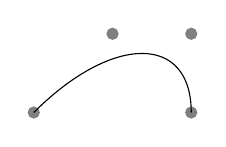
\begin{tikzpicture}
        \filldraw [gray] (0,0) circle [radius=2pt]
            (1,1) circle [radius=2pt]
            (2,1) circle [radius=2pt]
            (2,0) circle [radius=2pt];
        \draw (0,0) .. controls (1,1) and (2,1) .. (2,0);
    \end{tikzpicture}

    \begin{tikzpicture}
        \draw (-1.5,0) -- (1.5,0);
        \draw (0, -1.5) -- (0, 1.5);
        \draw (-1,0) .. controls (-1, 0.555) and (-0.555, 1) .. (0,1)
            .. controls (0.555, 1) and (1, 0.555) .. (1,0);
    \end{tikzpicture}

    \begin{tikzpicture}
        \draw (-1.5, 0) -- (1.5, 0);
        \draw (0, -1.5) -- (0, 1.5);
        \draw (0,0) circle[radius=1cm];
    \end{tikzpicture}

    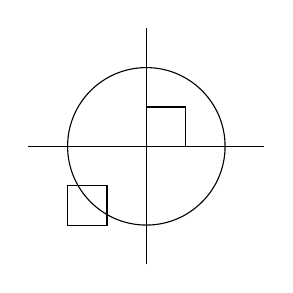
\begin{tikzpicture}
        \draw (-1.5, 0) -- (1.5, 0);
        \draw (0, -1.5) -- (0, 1.5);
        \draw (0,0) circle[radius=1cm];
        \draw (0,0) rectangle (0.5, 0.5);
        \draw (-0.5, -0.5) rectangle (-1,-1);
    \end{tikzpicture}

    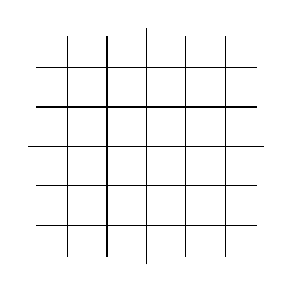
\begin{tikzpicture}
        \draw (-1.5, 0) -- (1.5, 0);
        \draw (0, -1.5) -- (0, 1.5);
        \draw[step=.5cm] (-1.4,-1.4) grid (1.4,1.4);
    \end{tikzpicture}

Styles are made even more powerful by parametrization (can also be 
used with a parameter).

    \tikzset{Karl's grid/.style={help lines, color=blue!50}}
    \tikzset{Karl's grid/.default=blue}
    \begin{tikzpicture}
        \draw[Karl's grid] (0,0) grid (1.5,2);
        \draw[Karl's grid=red] (2,0) grid (3.5,2);
    \end{tikzpicture}

    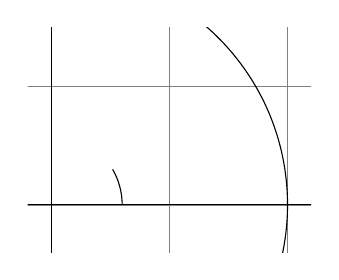
\begin{tikzpicture}[scale=3]
        \clip (-0.1, -0.2) rectangle (1.1, 0.75);
        \draw [step=.5cm, gray, very thin] (-1.4,-1.4) grid (1.4,1.4);
        \draw (-1.5,0) -- (1.5,0);
        \draw (0,-1.5) -- (0,1.5);
        \draw (0,0) circle [radius=1cm];
        \draw (3mm, 0mm) arc [start angle=0, end angle=30, radius=3mm];
    \end{tikzpicture}

\end{document}
